%%%%% This version of the MainThesis exists to help create piecewise chapters to upload as part of an annual review

% \documentclass[12pt, a4paper]{report}
% \usepackage[numbers]{natbib}
\usepackage{enumitem}
\usepackage{graphicx} % Required for inserting images
\usepackage{times}
\usepackage[utf8]{inputenc}
\usepackage{geometry} %%%
\geometry{a4paper, left=22mm,  top=22mm, bottom=22mm, right=22mm}
% \usepackage{stringstrings}
% \usepackage{ifthen}
\usepackage{array}
\usepackage[intoc]{nomencl}
\usepackage{lipsum} % for template filler text

% \usepackage{setspace}
% \usepackage[document]{ragged2e}
% \newcommand*\beginfrontmatter
    {\pagenumbering{roman}\setlength{\parskip}{0.5em}}

\newcommand*\frontmatter[1]
    {\newpage\thispagestyle{plain}\chapter*{#1}}

\newcommand*\beginmaincontent
    {\pagenumbering{arabic}\setcounter{page}{1}}

\newcommand*\maincontent[1]
    {\newpage\chapter{#1}}

\newcommand*\backmatter[1]
    {\newpage\chapter*{#1}}

    

\newcommand*\sectionisblank
    {\par\begin{center}\footnotesize{(this section is presently blank)}\end{center}\par\normalsize}

\newcommand*\sectionisincomplete
    {\par\begin{center}\footnotesize{(this section is presently incomplete)}\end{center}\par\normalsize}

\newcommand*\tobecompleted
    {\footnotesize{(to be completed)} \normalsize}

\newcommand*\sectionnote[1]
    {\par{\textbf{Note: } #1} \par \hrule \par \normalsize}

\newcommand*\makequote[2]
    {\vspace{2\baselineskip}
        \begin{quote}
            {\footnotesize #1}
        \end{quote}
    \hfill {\footnotesize #2} \hspace{4em}\normalsize}

\newcommand*\affil[1]
    {\textsuperscript{#1}}

\newcommand*\makelongaffil[4]
    {\vspace{\baselineskip}
    \begin{footnotesize}
    \noindent\textsuperscript{#1}#2\\ \phantom{\textsuperscript{#1}}#3\\\phantom{\textsuperscript{#1}}#4\par
    \end{footnotesize}}
    
\newcommand*\makeshortaffil[3]
    {\vspace{\baselineskip}
    \begin{footnotesize}
    \noindent\textsuperscript{#1}#2\\ \phantom{\textsuperscript{#1}}#3\par
    \end{footnotesize}}

% \setlength{\parskip}{0.5em}
% \setlength{\parindent}{10em}

\newcommand*\spacer[1]
    {\par\vspace*{#1\baselineskip}\par}

\renewcommand*\title[1]
    {\spacer{10} \begin{Large} \textbf{#1} \end{Large} \spacer{5}}
    
\renewcommand*\author[1]
    {presentado por \spacer{2} #1 \par}
    
\newcommand*\qualifications[1]
    {\par #1 \spacer{8}}

\newcommand*\degree[1]
{Presentado para cumplir con los requisitos del grado de \par #1 \spacer{6}}
        
\newcommand*\institution[2]
    {#1 \par}
    



% \begin{document}
% \begin{titlepage}
%     \centering  
%     \title{PhD title here} 
%     \author{Author Name}
%     \qualifications{Author Qualifications}
%     \degree{Doctor of Philosophy}
%     \institution{Deakin University}
%     \date{Month Year}
% \end{titlepage}

% \beginfrontmatter
% %%%%% --------- Abstract --------- %%%%%
% \frontmatter{Abstract}
% El deep learning ha revolucionado la reconstrucción de imágenes fotoacústicas a partir de datos crudos (raw data) provenientes de sensores, donde un eje representa el tiempo y el otro la dirección de escaneo. Las aproximaciones han evolucionado desde el uso de métodos convencionales complementados con deep learning para mejorar la calidad de imagen, hasta el desarrollo de redes neuronales que aprenden a reconstruir la imagen directamente desde los datos crudos. En este contexto, la arquitectura U-Net se ha convertido en un estándar de facto.
Sin embargo, el principal desafío al usar redes neuronales para la reconstrucción directa radica en la física subyacente del problema, que lo hace matemáticamente mal condicionado. Aunque existen métodos como las Physics Informed Neural Networks (PINN) para incorporar restricciones físicas, estos suelen ser computacionalmente costosos debido a las numerosas operaciones numéricas requeridas. En este trabajo, proponemos un nuevo marco de trabajo que permite a la red neuronal no solo reconstruir la imagen sino también mantener la consistencia física del problema.

Nuestra propuesta se basa en un enfoque inspirado en el data guided learning, que consta de dos fases principales. En la primera, entrenamos dos redes U-Net: una aprende a reconstruir imágenes a partir de datos crudos, mientras que la otra aprende el problema inverso, es decir, la generación de señales fotoacústicas a partir de imágenes, simulando así el proceso físico de propagación de ondas acústicas. En la segunda fase, realizamos un fine-tuning de la red de reconstrucción, incorporando la consistencia física como una restricción adicional en el proceso de aprendizaje. Este enfoque actúa como un supervisor que guía a la red para que no solo aprenda a reconstruir imágenes con alta calidad, sino que también respete los principios físicos fundamentales del proceso fotoacústico.

% %%%%% ----- Acknowledgements ----- %%%%%
% \frontmatter{Acknowledgements}
% 
\sectionisblank

% %%%%% -- Contribution Statement -- %%%%%
% \frontmatter{Contribution statement}

% \subsection*{Declaration by author}\sectionisincomplete

% \subsection*{Supervisors}
% Title. Supervisor One\affil{1}, Title. Supervisor Two\affil{2}, Title. Supervisor Three\affil{1}, and Title. Supervisor Four\affil{3,4}

% \makelongaffil{1}{A \textit{long} affiliation (e.g., School)}{allows for three (e.g., Faculty)}{lines to be specified (e.g., Institution)}
% \makeshortaffil{2}{A \textit{short} affiliation (e.g., Department)}{only has two (e.g., Company)}
% \makeshortaffil{3}{A supervisor may have}{multiple affiliations}
% \makeshortaffil{4}{An affiliation may be used by}{multiple supervisors}


% %%%%% ----- Publications ----- %%%%%
% \frontmatter{List of publications}
% \sectionisincomplete

% \subsection*{Publications included in this thesis}
% \tobecompleted

% \subsection*{Submitted manuscripts included in this thesis}
% \tobecompleted

% \subsection*{Other publications during candidature}
% \tobecompleted


% % %%%%% ---- Ethics Statement ----- %%%%%
% % \frontmatter{Ethics approvals}
% % \sectionisincomplete

% %%%%% ---- Table of Contents ---- %%%%%
% \tableofcontents

% %%%%% ----- List of Figures ----- %%%%%
% \listoffigures

% %%%%% ----- List of Tables ------ %%%%%
% \listoftables

% %%%%% -- List of Abbreviations -- %%%%%
% \makenomenclature
\renewcommand{\nomname}{List of Abbreviations}

\nomenclature{AI}{Artificial Intelligence}


% \printnomenclature

% \beginmaincontent
% %%%%% ------ Introduction ------ %%%%%
% \maincontent{Introduction}
% \section{Introducción}

En la actualidad, las técnicas de imagen médica no invasivas han revolucionado el diagnóstico y tratamiento de enfermedades. Entre estas técnicas emergentes, la imagen fotoacústica (PAI, por sus siglas en inglés) se destaca por su capacidad única de combinar el contraste óptico con la resolución ultrasónica, permitiendo visualizar estructuras biológicas con un nivel de detalle sin precedentes.

La reconstrucción de imágenes fotoacústicas representa un desafío significativo debido a la complejidad de los fenómenos físicos involucrados y la presencia inherente de ruido en las señales adquiridas. Los métodos tradicionales de reconstrucción, basados en aproximaciones analíticas y técnicas iterativas, a menudo resultan computacionalmente costosos y pueden producir artefactos en las imágenes reconstruidas.

En este contexto, las arquitecturas de aprendizaje profundo, específicamente las redes neuronales convolucionales (CNNs), han demostrado un potencial extraordinario para abordar estos desafíos. Sin embargo, un desafío fundamental persiste: la incorporación efectiva de las restricciones físicas del problema en el proceso de aprendizaje. Nuestro trabajo se centra en el desarrollo de un marco de trabajo innovador que permite a las redes neuronales aprender simultáneamente la reconstrucción de imágenes y mantener la consistencia física del problema.

\section{Preguntas de Investigación y Contribuciones}
\label{sec:prop}

Este trabajo de investigación se centra en el desarrollo de un marco de trabajo de aprendizaje profundo que optimice simultáneamente la calidad de reconstrucción y la consistencia física en imágenes fotoacústicas. Para lograr este objetivo, se plantean las siguientes preguntas de investigación:

\subsection{Preguntas de Investigación}
\label{sec:ques}

La pregunta principal de investigación es la siguiente:
\begin{quote}
\textit{¿Cómo podemos desarrollar un marco de trabajo de aprendizaje profundo que optimice simultáneamente la calidad de reconstrucción y la consistencia física en imágenes fotoacústicas?}
\end{quote}

Para abordar esta pregunta de manera sistemática, se han establecido las siguientes sub-preguntas:

\begin{enumerate}[start=1,label={PI\arabic*:},wide = 0pt, leftmargin = 3em]
\item \textit{¿Cómo podemos desarrollar una arquitectura de red neuronal que incorpore el conocimiento físico del proceso fotoacústico, considerando tanto la complejidad del entrenamiento como la eficiencia computacional que limita a los métodos PINN tradicionales?}
\item \textit{¿Qué ventajas ofrece el aprendizaje del problema inverso en la consistencia física de la reconstrucción?}
\item \textit{¿Cuál es el impacto del fine-tuning con restricciones físicas en la calidad final de la reconstrucción?}
\item \textit{¿Cómo se comporta el método propuesto en términos de robustez y generalización?}
\end{enumerate}

\subsection{Contribuciones}
\label{sec:cont}

Esta investigación proporciona las siguientes contribuciones al conocimiento:

\begin{enumerate}[start=1,label={C\arabic*:},wide = 0pt, leftmargin = 3em]
\item Un marco de trabajo innovador que integra el aprendizaje de la física del problema mediante una arquitectura dual de redes U-Net.
\item Una metodología de fine-tuning que balancea efectivamente la calidad de reconstrucción con la consistencia física, demostrada por mejoras cuantificables:
    \begin{itemize}
        \item Reducción del 18.6\% en MSE de reconstrucción
        \item Mejora del 18.8\% en consistencia física de señales
        \item Incremento en SSIM hasta 0.973
    \end{itemize}
\item Una implementación computacionalmente eficiente que aborda las limitaciones de los métodos PINN tradicionales mediante un enfoque de redes duales, reduciendo la complejidad del entrenamiento mientras preserva la consistencia física del problema.
\item Un conjunto completo de experimentos y evaluaciones que validan la efectividad del método propuesto.
\item Una implementación de código abierto del modelo propuesto y sus herramientas asociadas.
\end{enumerate}

\section{Estructura de la Tesis}
\label{sec:thes}

El formato de esta tesis es por publicación, por lo que se busca publicar esta investigación en los siguientes artículos:

\begin{enumerate}[start=1,label={P\arabic*:},wide = 0pt, leftmargin = 3em]
\item Un Marco de Trabajo Physics-Guided para la Reconstrucción de Imágenes Fotoacústicas (PI1; C1)
\item Análisis del Impacto de la Consistencia Física en la Reconstrucción de PAI (PI2; C2)
\item Optimización del Fine-tuning con Restricciones Físicas en PAI (PI3; C3, C4)
\item Evaluación de Robustez y Generalización en Reconstrucción PAI con Guía Física (PI4; C5)
\end{enumerate}

% %%%%% ---- Literature Review ---- %%%%%
% \maincontent{Literature review}
% Esta revisión de literatura abarca dos áreas principales de investigación: la imagen fotoacústica y las técnicas de aprendizaje profundo para la reconstrucción de imágenes médicas \cite{valluru2016molecular}. El objetivo es establecer una base sólida para entender el estado actual de la tecnología fotoacústica y las aplicaciones más recientes de redes neuronales, específicamente las arquitecturas basadas en atención, en el campo de la reconstrucción de imágenes médicas.

La revisión abarca publicaciones desde 2015 hasta 2024, con énfasis especial en los avances más recientes en arquitecturas de deep learning para procesamiento de imágenes médicas \cite{shen2017deep}. Se han incluido trabajos tanto teóricos como experimentales, con particular atención a aquellos que abordan los desafíos específicos de la reconstrucción fotoacústica \cite{antholzer2019deep}.
\section{Imagen Fotoacústica: Fundamentos y Avances} \label{sec:lit:first}

Para enteder la imagen fotoacústica, es necesario comprender los principios físicos y tecnológicos subyacentes, así como los métodos tradicionales de reconstrucción utilizados en la práctica clínica actual \cite{wang2012photoacoustic}. A continuación, se presentan los aspectos más relevantes de la imagen fotoacústica y su evolución en los últimos años.

\subsection{Principios Físicos y Tecnológicos} \label{sec:lit:first:one}
El efecto fotoacústico, descubierto por Alexander Graham Bell en 1880, se fundamenta en la generación de ondas acústicas mediante la absorción de energía electromagnética pulsada \cite{bell1880production}. En el contexto de imagen médica, este fenómeno permite obtener información tanto estructural como funcional del tejido biológico \cite{xu2006photoacoustic}. La técnica combina la alta resolución espacial de los ultrasonidos con el alto contraste de la imagen óptica, superando las limitaciones individuales de ambas modalidades \cite{wang2012photoacoustic}.

Los sistemas modernos de imagen fotoacústica utilizan láseres pulsados de nanosegundos para generar ondas ultrasónicas en el tejido \cite{li2021photoacoustic}. La absorción de energía lumínica produce una expansión termoelástica local que genera ondas de presión detectables mediante transductores ultrasónicos \cite{wang2016review}. Esta información se procesa posteriormente para reconstruir la distribución espacial de los absorbentes ópticos en el tejido (ver Figura \ref{fig:efecto_fotoacustico}).

\begin{figure}[H]
    \centering
    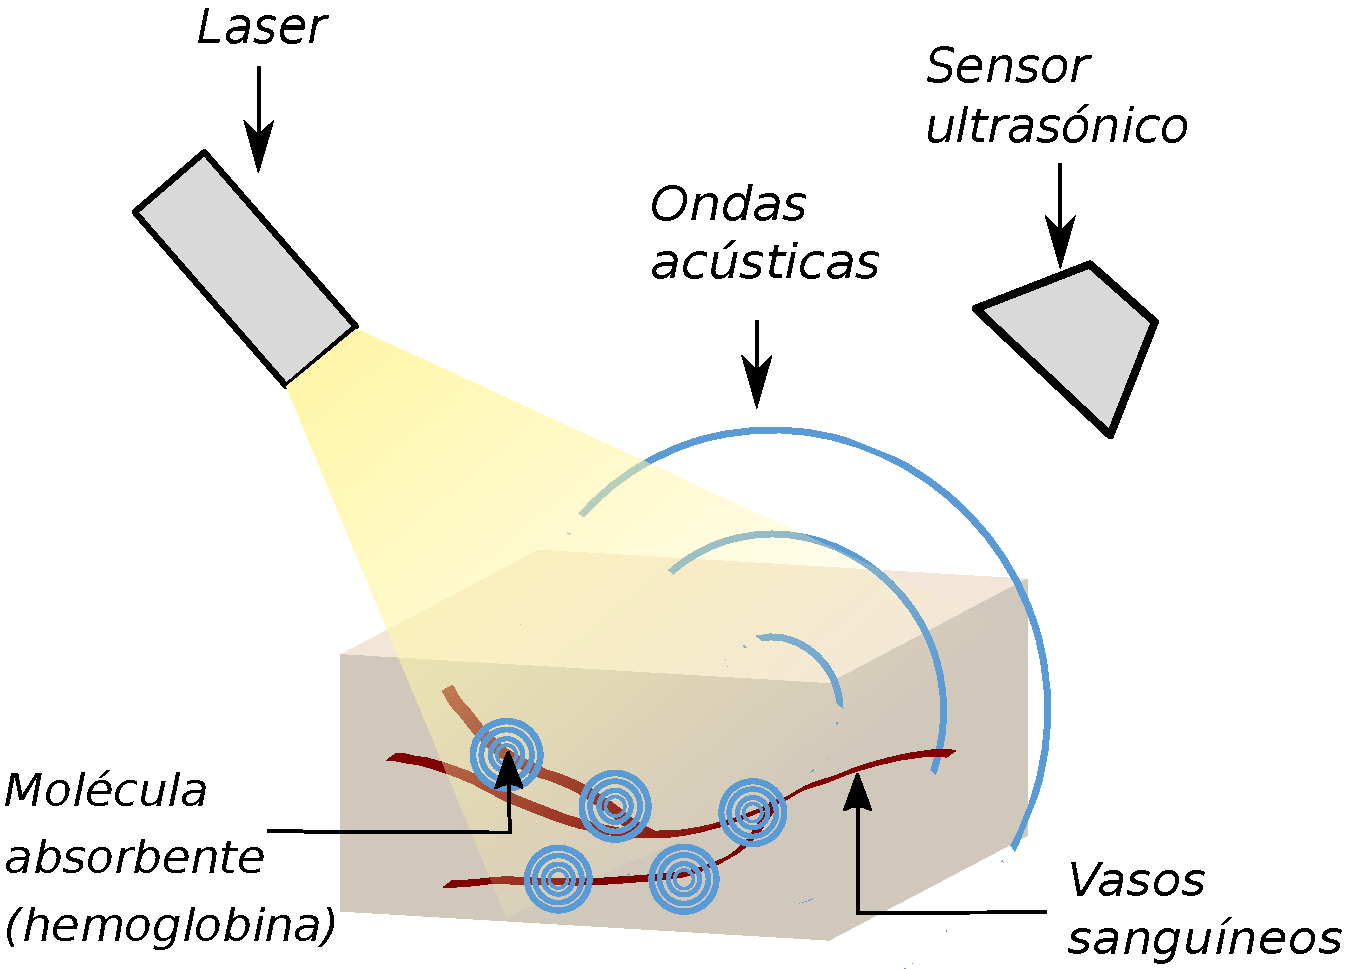
\includegraphics[width=\textwidth]{Images/effect.pdf}
    \caption{Efecto fotoacústico.}
    \label{fig:efecto_fotoacustico}
\end{figure}

Las aplicaciones clínicas actuales incluyen la detección temprana de cáncer, imagen funcional cerebral, y caracterización vascular, entre otras \cite{kim2021clinical}. Los avances recientes en tecnología de sensores y sistemas de adquisición han mejorado significativamente la calidad y velocidad de adquisición de datos fotoacústicos \cite{zhang2020advances}.
\subsection{Métodos Tradicionales de Reconstrucción} \label{sec:lit:first:two}
Los métodos convencionales de reconstrucción fotoacústica se pueden clasificar en tres categorías principales \cite{kuchment2008mathematics}:

Los métodos analíticos, como la retroproyección filtrada y las técnicas de transformada de Fourier, proporcionan soluciones directas basadas en la ecuación de onda fotoacústica \cite{xu2005universal}. Estos métodos son computacionalmente eficientes pero pueden generar artefactos significativos en condiciones no ideales.

Los métodos iterativos, incluyendo técnicas de optimización variacional y métodos algebraicos, ofrecen mayor flexibilidad para incorporar información a priori y restricciones físicas \cite{huang2013full}. Sin embargo, su alto costo computacional limita su aplicabilidad en escenarios clínicos en tiempo real.

Los métodos basados en modelos incorporan explícitamente la física del problema mediante simulaciones numéricas detalladas \cite{cox2009challenges}. Aunque precisos, estos métodos requieren un conocimiento exacto de los parámetros físicos del medio y son computacionalmente intensivos.

% -----------------------------------------------------
\section{Importancia de la Consistencia Física en Reconstrucción Fotoacústica}

La consistencia física en la reconstrucción de imágenes fotoacústicas ha emergido como un aspecto crítico para obtener resultados robustos y fiables \cite{hauptmann2018model}. Esta importancia se fundamenta en múltiples aspectos que impactan tanto la calidad de la reconstrucción como la fiabilidad del resultado para aplicaciones prácticas.


\subsection{Naturaleza del Problema Inverso}
El problema inverso fotoacústico es inherentemente mal condicionado \cite{wang2009inverse}, lo que significa que pequeñas perturbaciones en los datos de entrada (señales acústicas) pueden resultar en grandes variaciones en la solución. La incorporación de restricciones físicas actúa como una forma natural de regularización \cite{arridge2016solving}, ayudando a:

\begin{itemize}
    \item Reducir el espacio de soluciones posibles a aquellas que son físicamente plausibles.
    \item Estabilizar el proceso de reconstrucción frente al ruido y las incertidumbres en las mediciones \cite{antholzer2019deep}.
    \item Mejorar la unicidad de la solución al incorporar información a priori sobre el comportamiento físico del sistema.
\end{itemize}

\subsection{Garantías de Validez y Robustez}
La consistencia física proporciona garantías importantes sobre la validez de las reconstrucciones \cite{shan2019physics}:

\begin{itemize}
    \item Asegura que las imágenes reconstruidas no solo sean visualmente plausibles, sino que también representen estados físicamente posibles del sistema.
    \item Permite verificar que la reconstrucción obedece las leyes fundamentales de la fotoacústica, como la ecuación de onda y las condiciones de contorno \cite{tick2016image}.
    \item Mejora la robustez del método, especialmente en casos con datos limitados o ruidosos \cite{hauptmann2020deep}.
\end{itemize}

\subsection{Ventajas en el Aprendizaje Profundo}
En el contexto del aprendizaje profundo, la incorporación de la física ofrece ventajas significativas \cite{raissi2019physics}:

\begin{itemize}
    \item Reduce la dependencia de grandes conjuntos de datos de entrenamiento al incorporar conocimiento previo sobre la física del problema \cite{hoffer2019augmented}.
    \item Proporciona una guía natural para el proceso de optimización, ayudando a la red a converger a soluciones más significativas \cite{zhou2020physics}.
    \item Permite detectar y corregir reconstrucciones que, aunque visualmente plausibles, violan las leyes físicas fundamentales del sistema.
\end{itemize}


\section{Deep Learning en Reconstrucción de Imágenes Fotoacústicas}

El aprendizaje profundo ha demostrado un éxito extraordinario en reconstrucción de imágenes fotoacústicas, particularmente con la arquitectura U-Net. Sin embargo, un desafío fundamental persiste: cómo incorporar efectivamente el conocimiento físico del problema en el proceso de aprendizaje.

\subsection{Evolución de Métodos de Reconstrucción con Deep Learning}

Las primeras aproximaciones utilizaban redes neuronales como post-procesamiento para mejorar imágenes reconstruidas con métodos tradicionales. Sin embargo, trabajos recientes como el de Guan et al. \cite{guan2020fully}, han demostrado que las arquitecturas densamente conectadas pueden abordar directamente el problema de reconstrucción, especialmente en casos de muestreo disperso donde los métodos tradicionales generan artefactos significativos.

\subsection{Incorporación de Física en Redes Neuronales}

La incorporación de conocimiento físico en redes neuronales ha seguido principalmente dos enfoques:

\begin{itemize}
\item \textbf{Physics-Informed Neural Networks (PINNs):} Incorporan directamente las ecuaciones diferenciales en la función de pérdida. Sin embargo, como se discute en \cite{Zhou2024DataGuided}, estos métodos pueden enfrentar desafíos durante el entrenamiento debido al desbalance entre los términos de pérdida física y de datos.

\item \textbf{Data-Guided Physics-Informed Approaches:} Propuestos más recientemente, estos métodos buscan un balance entre el aprendizaje basado en datos y las restricciones físicas. El trabajo de Zhou et al. \cite{Zhou2024DataGuided} introduce un marco de trabajo en dos fases que primero optimiza la pérdida de datos y luego incorpora gradualmente las restricciones físicas.
\end{itemize}

\subsection{Desafíos en la Incorporación de Física}

La incorporación de restricciones físicas en redes neuronales para reconstrucción fotoacústica presenta varios desafíos únicos:

\begin{itemize}
\item \textbf{Complejidad Computacional:} Los métodos PINN tradicionales requieren la evaluación de derivadas durante el entrenamiento, lo que aumenta significativamente el costo computacional.

\item \textbf{Balance de Pérdidas:} Como se evidencia en \cite{Zhou2024DataGuided}, mantener un balance adecuado entre la pérdida de datos y las restricciones físicas es crucial para el entrenamiento efectivo.

\item \textbf{Naturaleza Mal Condicionada:} El problema inverso en fotoacústica es inherentemente mal condicionado, lo que complica la incorporación de restricciones físicas.
\end{itemize}

\section{Limitaciones y Desafíos Actuales}

Los métodos actuales de incorporación de física en redes neuronales enfrentan varios desafíos:

\begin{itemize}
\item \textbf{Eficiencia Computacional:} Los PINN tradicionales son computacionalmente costosos, limitando su aplicabilidad en escenarios clínicos.

\item \textbf{Generalización:} La mayoría de los conjuntos de datos son simulados, planteando preguntas sobre la generalización a casos reales.

\item \textbf{Validación:} La evaluación de la consistencia física en las reconstrucciones requiere métricas específicas que van más allá de las medidas de calidad de imagen tradicionales.
\end{itemize}

Estos desafíos motivan la búsqueda de nuevos enfoques que puedan mantener la consistencia física mientras son computacionalmente eficientes y robustos en aplicaciones reales.

% %%%%% ------- Paper 1 ------- %%%%%
% \setcounter{chapter}{2}
% \maincontent{This is the full title of my first paper}
% \input{3_PaperOne}

% %%%%% ----- Paper 2 ----- %%%%%
% \setcounter{chapter}{3}
% \maincontent{This is where I would put my second paper \textit{\textbf{if I had any}}}
% \input{4_PaperTwo}

% %%%%% -------- Paper 3 -------- %%%%%
% \setcounter{chapter}{4}
% \maincontent{Paper three is basically the Thursday of your thesis}
% \input{5_PaperThree}

% %%%%% ------ Paper 4 ------ %%%%%
% \setcounter{chapter}{5}
% \maincontent{Congratulations, Doctor.}
% \input{6_PaperFour}

% %%%%% ------ Paper 5 ------ %%%%%
% \setcounter{chapter}{6}
% \maincontent{Okay, nobody likes a show-off}
% \input{7_PaperFive}

% % %%%%% ------ Conclusion ------ %%%%%
% \setcounter{chapter}{7}
% \maincontent{Summary, discussion, and future directions}
% \input{9_Conclusion}

% %%%%% ------ References ------ %%%%%
% % \backmatter{References}
% \bibliography{references.bib} %%All bibtex references are in references.bib file
% \bibliographystyle{abbrv}

% \end{document}